\subsection{Hidrodinámica}

\begin{frame}{Flotabilidad (hidrostática)}

\begin{center}
$\Delta = \rho \nabla$
\end{center}

$\Delta = $ Desplazamiento (peso del objeto)

$\rho = $ Densidad del agua

$\nabla = $ Volumen de agua desplazada

\begin{figure}
  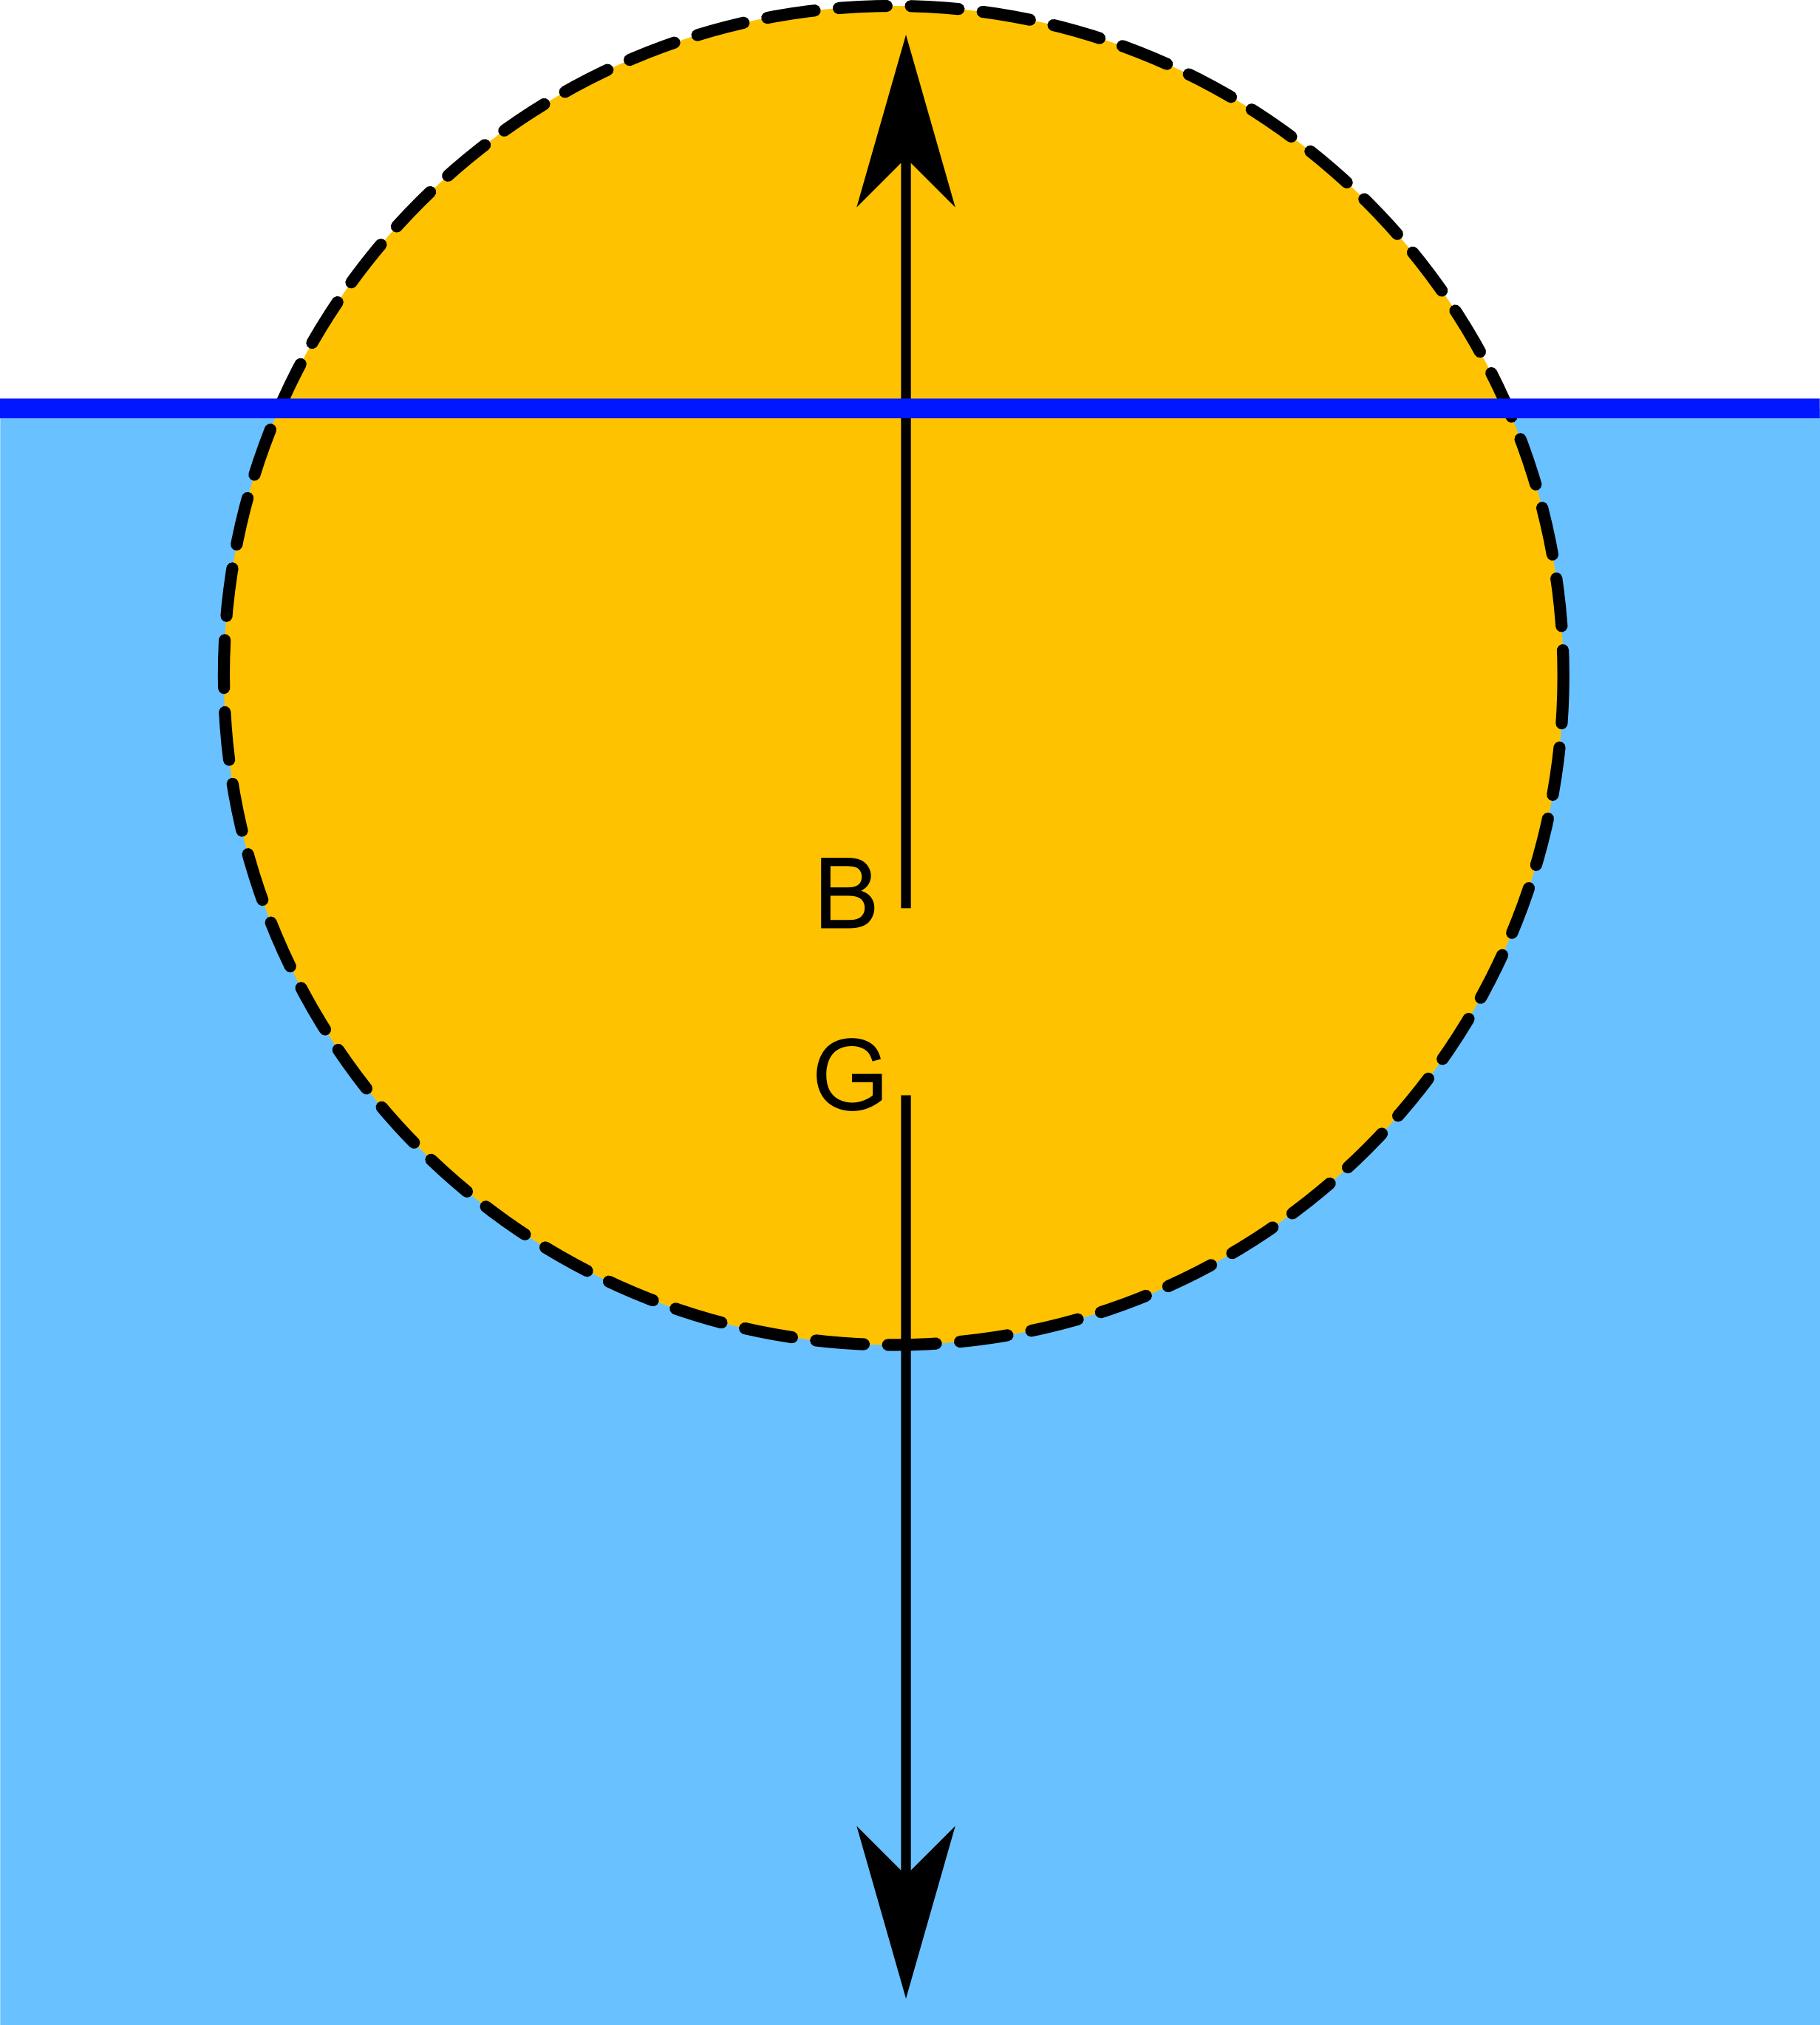
\includegraphics[scale=0.15]{archimedes} 
\end{figure}

\pause

\begin{center}
$\nabla = \frac{\pi}{3} \left( R - z \right)^2 \left( 2 R + z \right)$
\end{center}

$R = $ Radio de la esfera

$z = $ Altura del centro de la esfera con respecto de la superficie libre

\end{frame}

\begin{frame}{Flotabilidad (hidrodinámica)}

\begin{center}
$\frac{\partial^2 z}{\partial t^2} = \vert \mathbf{g} \vert \left( \Delta - \rho \nabla \right)
= f(z^3)
$
\end{center}

Movimiento no amortiguado, es decir, el objeto nunca llegará a estar en
equilibirio.
%
Lo solucionamos añadiendo un término amortiguador:

\begin{center}
$\frac{\partial^2 z}{\partial t^2} = \vert \mathbf{g} \vert \left( \Delta - \rho \nabla \right)
- K \Delta^{2/3} \left(\frac{\partial z}{\partial t}\right)^3$
\end{center}

Podemos usar el mismo término amortiguador para todos los movimientos en $x$,
$y$ y $z$.

\end{frame}

\begin{frame}{Estabilidad}

Excitación del mar del tipo:

\begin{center}
$M = A \cdot \cos\left( \omega t \right)$
\end{center}

Estabilidad regida por el parámetro $GM$:

\begin{figure}
  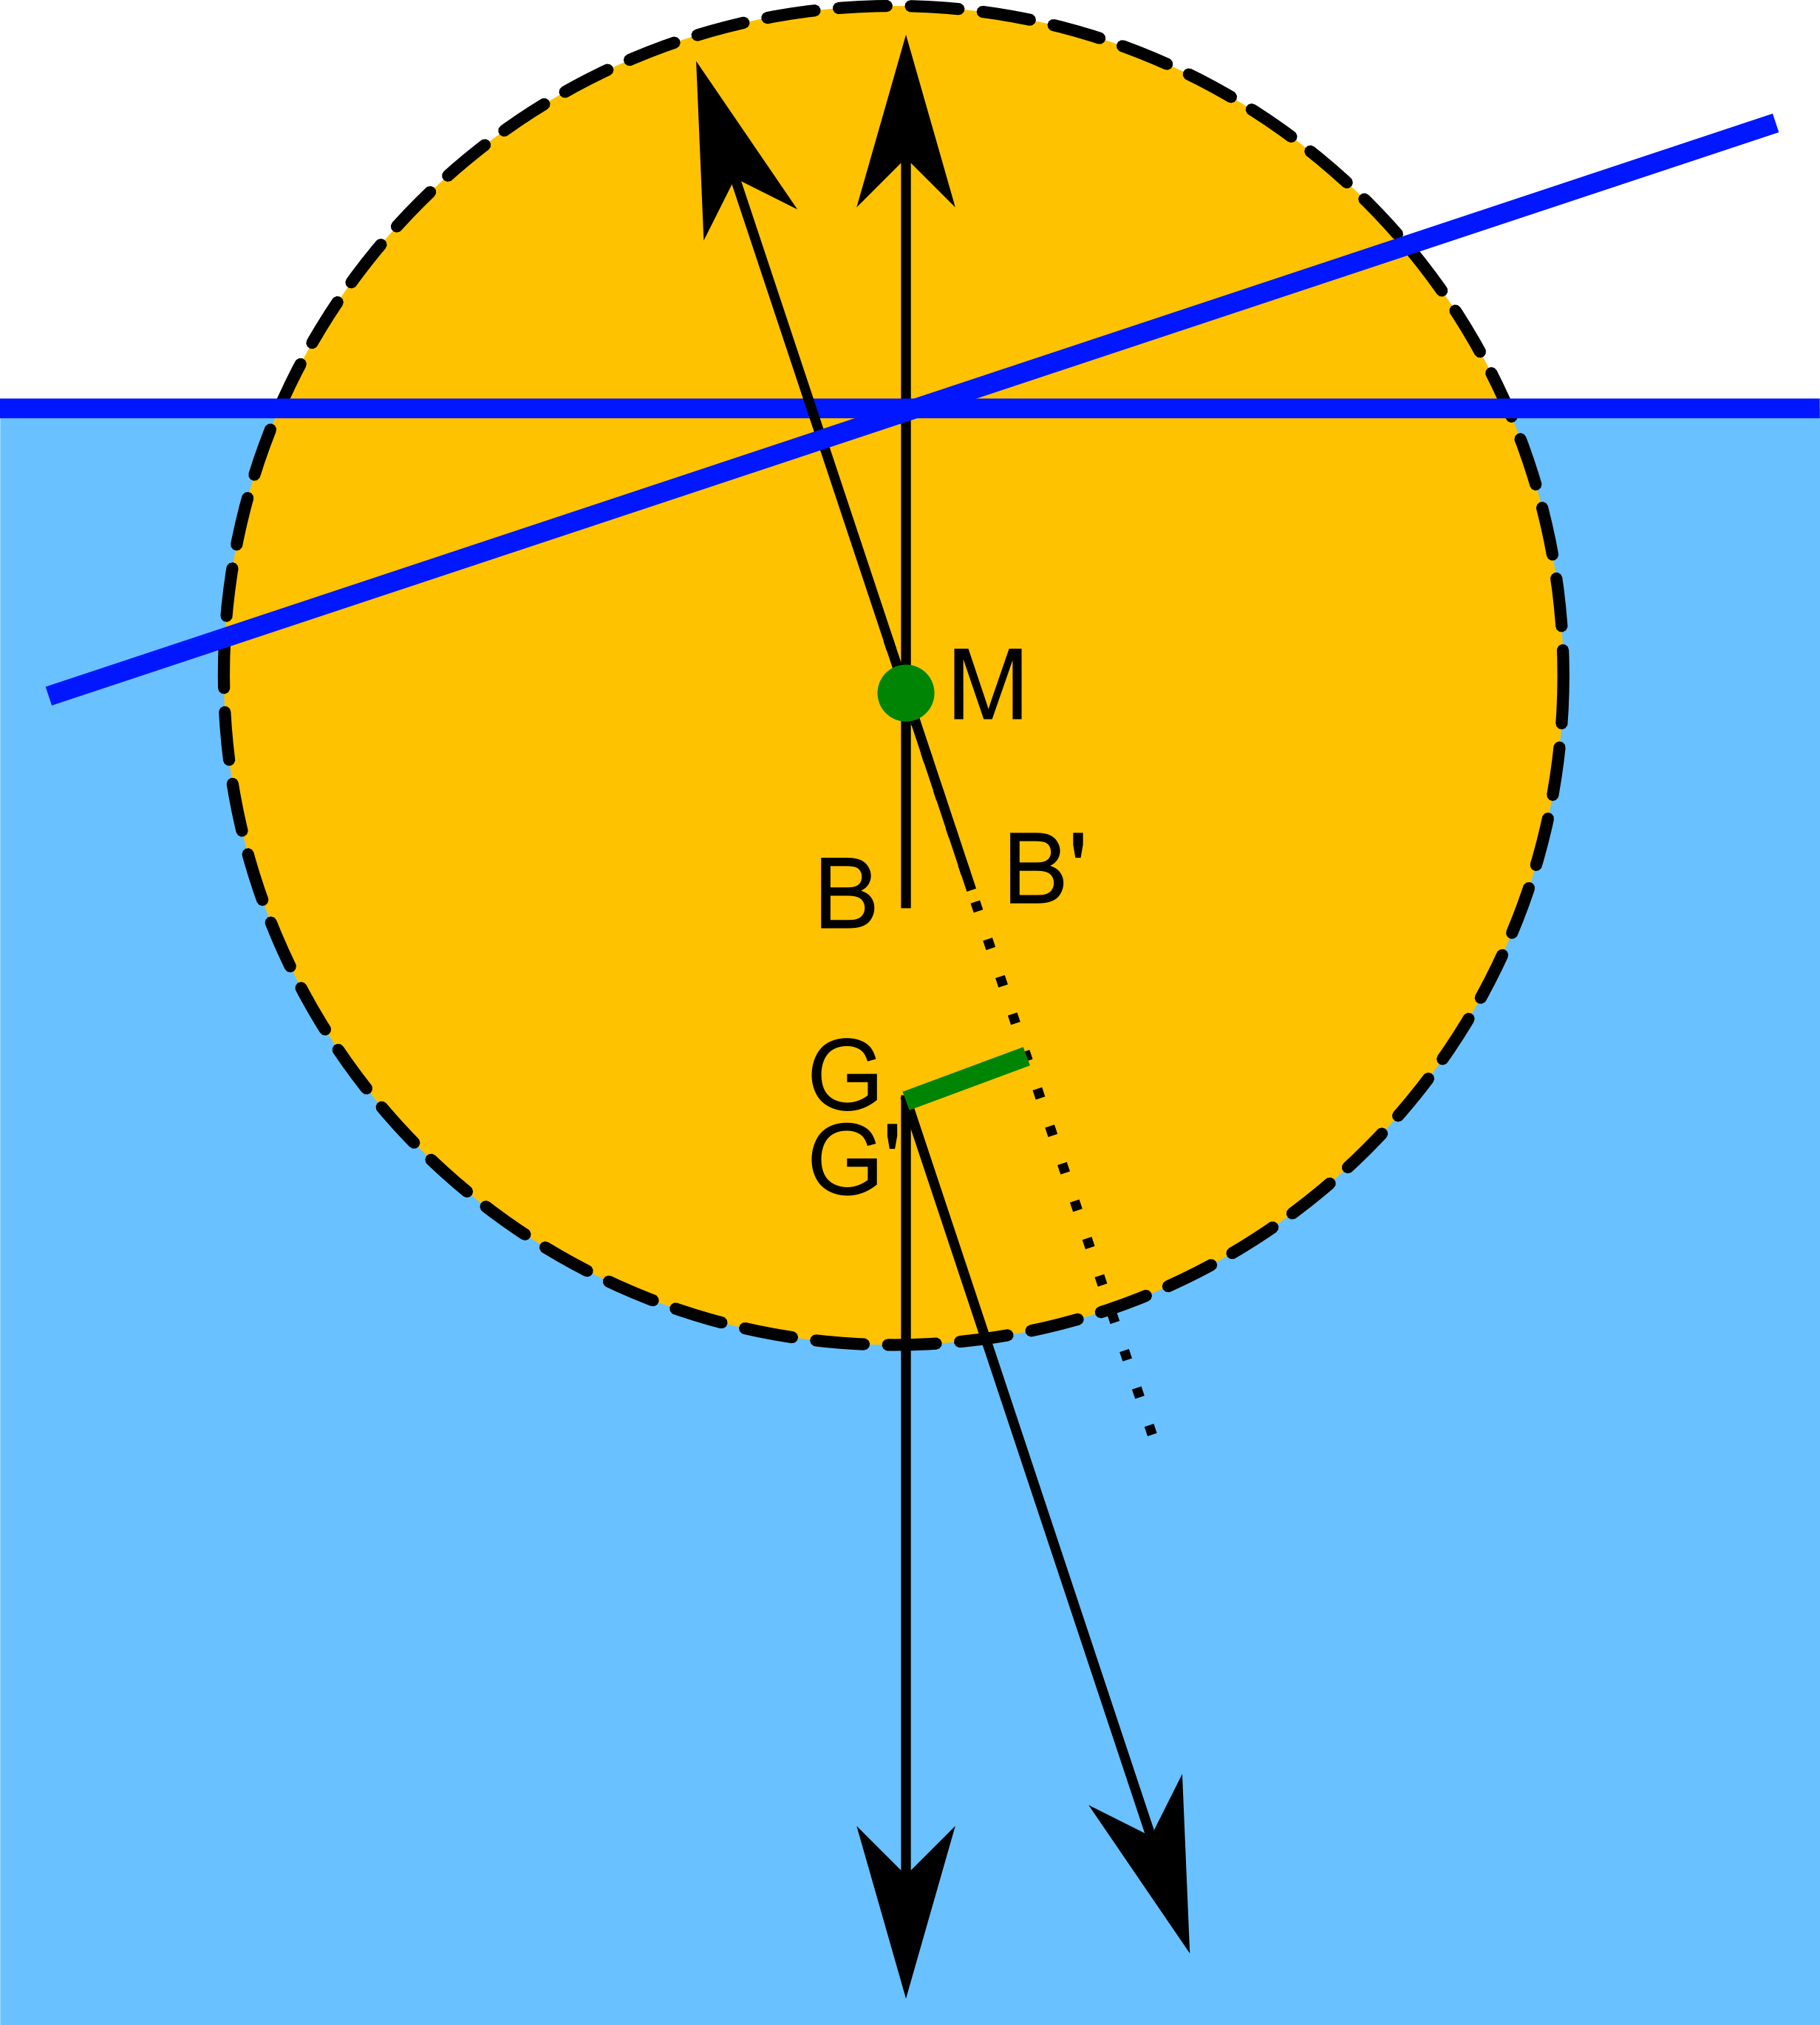
\includegraphics[scale=0.15]{stability} 
  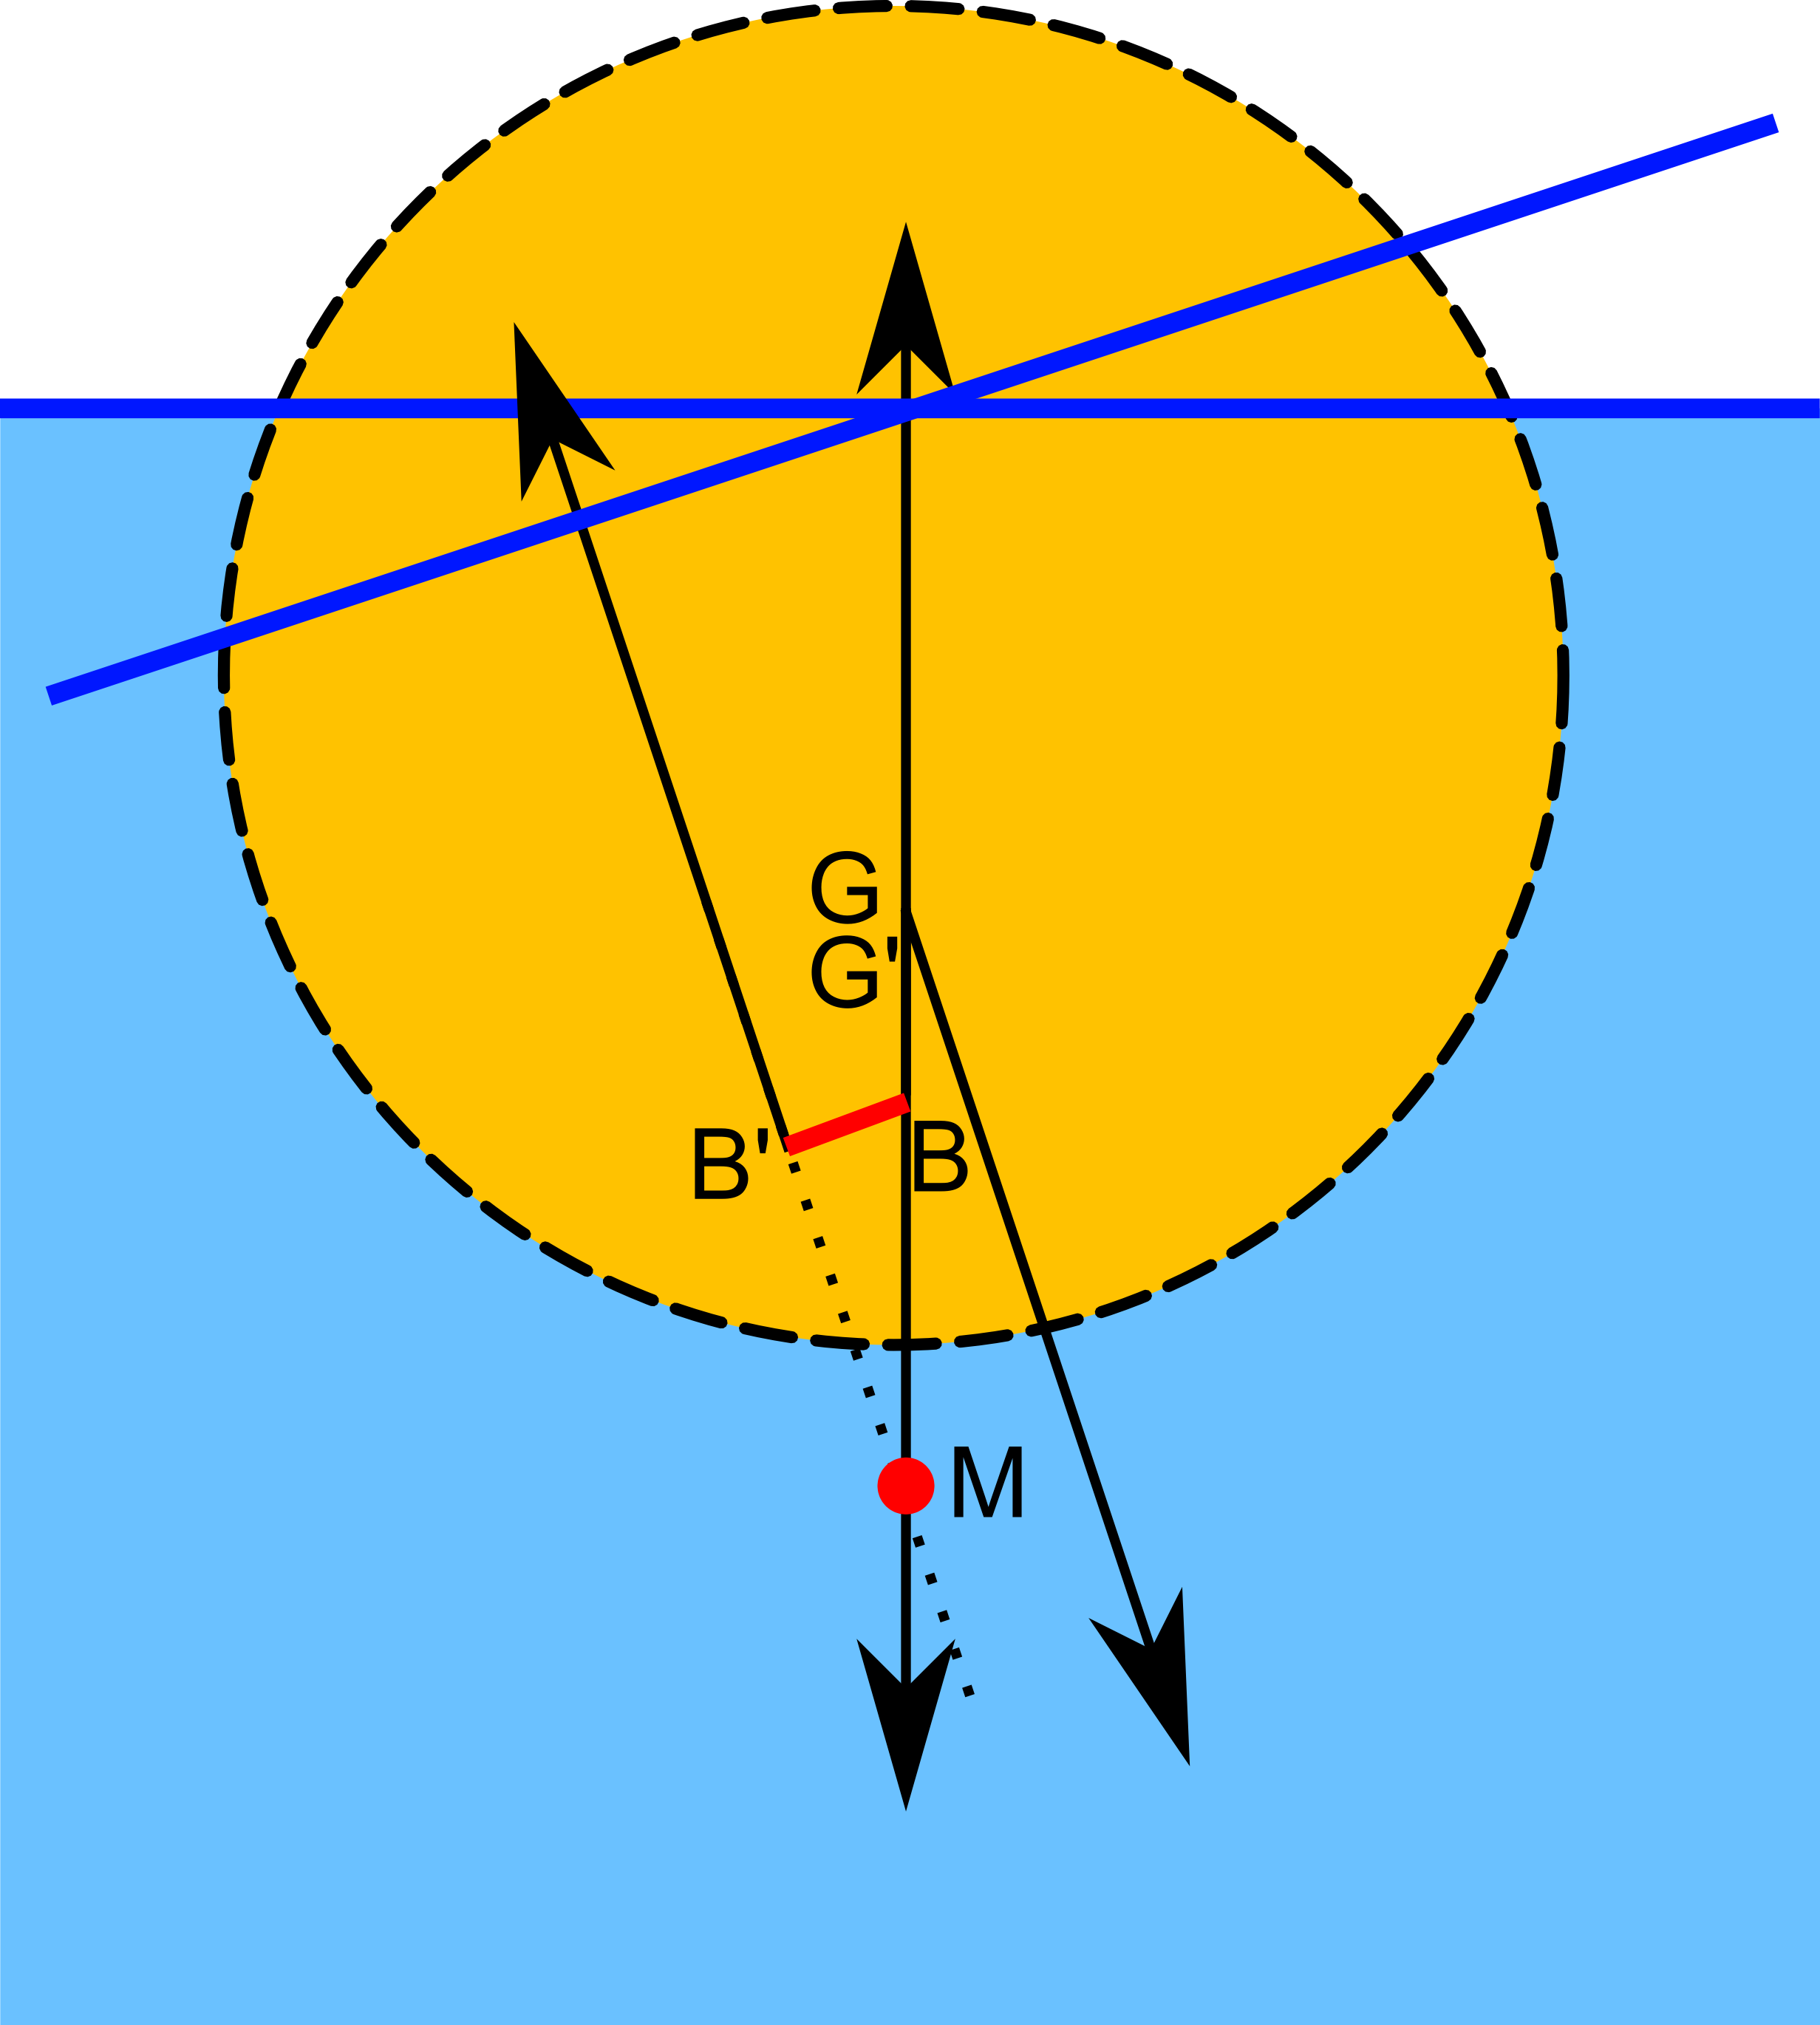
\includegraphics[scale=0.15]{stability_bad} 
\end{figure}

\pause

\begin{center}
$M = \vert \mathbf{g} \vert \Delta GM \sin\left( \theta \right)$
\end{center}

\pause

$\vert \left. \mathbf{u_x} \right\vert_{local}
\cdot
\vert \left. \mathbf{u_x} \right\vert_{global} = \cos\left( \theta \right)
\longrightarrow
\vert \left. \mathbf{u_x} \right\vert_{local}
\cdot
\vert \left. \mathbf{u_z} \right\vert_{global} = \sin\left( \theta \right)$

En este caso también añadimos un término viscoso.

\end{frame}
